\subsubsection{Symmetrie zur Quadrantenhalbierenden}

\begin{figure}[H]
    \centering
    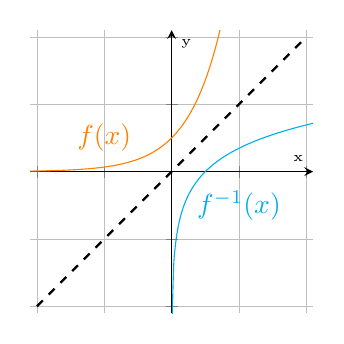
\begin{tikzpicture}
        \begin{axis}[
            unit vector ratio*=1 1 1,
            xmin=-4.2, xmax=4.2,
            ymin=-4.2, ymax=4.2,
            width=6cm,
            grid=both,
            axis lines=middle,
            grid style={line width=.1pt, draw=gray!20},
            major grid style={line width=.2pt,draw=gray!50},    
            ticklabel style={font=\tiny},
            xticklabels={,,},
            yticklabels={,,},
            xlabel style={font=\tiny},
            ylabel style={font=\tiny},
            xlabel={x}, ylabel={y}
            ]
            \draw [orange, smooth, samples=100] plot (\x, {exp(\x)});
            \draw [cyan, smooth, samples=100, domain=1/100:5] plot (\x,
            {ln(\x)});
            \draw[dashed, thick] (-4,-4) -- (4,4);
            \node[orange] at (axis cs: -2, 1) {\( f(x) \)};
            \node[cyan] at (axis cs: 2, -1) {\( f^{-1}(x) \)};
        \end{axis}
    \end{tikzpicture}
    \caption{Symmetrie zur Quadrantenhalbierenden}\label{fig:symquadrantenhalbierende}
\end{figure}

\subsubsection{Umkehrfunktion}

\[
    f^{-1}(x) \neq \frac{1}{f(x)}
\]

\(^{-1}\) steht für die Umkehrfunktion und nicht für eine \(-1\) im Exponenten.

\begin{figure}[H]
    \centering
    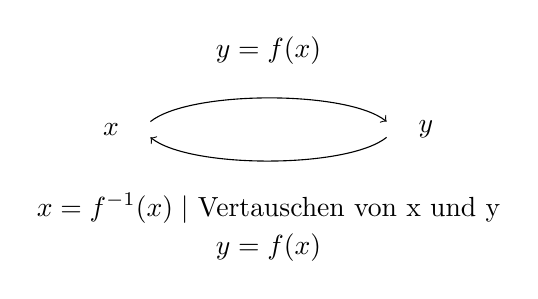
\begin{tikzpicture}
      \node at (-2,0) {\(x\)};
      \node at (2,0) {\(y\)};
      \draw[->] (-1.5,0.1) .. controls (-1,0.5) and (1,0.5) .. (1.5,0.1);
      \draw[<-] (-1.5,-0.1) .. controls (-1,-0.5) and (1,-0.5) .. (1.5,-0.1);
      \node at (0, 1) {\(y = f(x)\)};
      \node at (0, -1) {\(x = f^{-1}(x) \mid \) Vertauschen von x und y};
      \node at (0, -1.5) {\(y=f(x)\)};
    \end{tikzpicture}
\end{figure}

\begin{align*}
    f &= \{ (x,y) \mid x \in D_f, y \in W_f, y = f(x) \} \\
    f^{-1} &= \{ (y,x) \mid y \in D_f^{-1} = W_f, x \in W_f^{-1}, x = f^{-1}(y) \} \\
    \Rightarrow f^{-1} &= \{ (x,y) \mid x \in D_f^{-1} = W_f, y \in W_f^{-1}, y = f^{-1}(x) \}
\end{align*}

\paragraph{Rechenrezept}

\begin{itemize}
    \item \(x\) und \(y\) vertauschen
    \item \(x = f(y)\) nach \(y\) auflösen
\end{itemize}

\paragraph{Beispiel}

\begin{align*}
    y &= f(x) = 2x - 1 \\
    x &= 2y - 1 \\
    y &= \frac{x + 1}{2}
\end{align*}

\begin{figure}[H]
    \centering
    \begin{tikzpicture}
        \begin{axis}[
            defaultnonumbers,
            xmin=-4.2, xmax=4.2,
            ymin=-4.2, ymax=4.2,
            width=4.4cm
            ]
            \draw[orange] plot (\x, {2 * \x - 1});
            \draw[cyan] plot (\x, {(\x + 1) / 2 });
            \draw[dashed] (-4,-4) -- (4,4);
            \node[orange] at (axis cs: 2, -1) {\( f(x) \)};
            \node[cyan] at (axis cs: -2, 1) {\( f^{-1}(x) \)};
        \end{axis}
    \end{tikzpicture}
\end{figure}

% BILD
% x^2 und sqrt(x)

\paragraph{Beispiele}

\subparagraph{1. Beispiel (siehe Abb.~\ref{fig:beispiel1_umkehrfunktion})}

\begin{align*}
    y = f(x) &= \frac{5x}{x+1} -2 \\
    x &= \frac{5y}{y+1} -2 &&\mid +2 \\
    x+2 &= \frac{5y}{y+1} &&\mid  \cdot (y + 1) \\
    (x+2)(x+1) &= 5y \\
    xy + x + 2y + 2 &= 5y &&\mid -xy-2y \\
    x + 2 &= 5y -xy -2y \\
    x + 2 &= y (5-x -2 ) &&\mid : (2-x) \\
    y &= \frac{x+2}{3-x} = f^{-1}(x)
\end{align*}

\begin{figure}[H]
    \centering
    \begin{tikzpicture}
        \begin{axis}[
            defaultnonumbers,
            xmin=-10.2, xmax=10.2,
            ymin=-10.2, ymax=10.2,
            width=6.4cm
            ]
            \draw[orange, smooth, samples=100, domain=-10:-1-1/10] plot (\x, {(5*\x)/(\x + 1)-2});
            \draw[orange, smooth, samples=100, domain=-1+1/10:10] plot (\x, {(5*\x)/(\x + 1)-2});
            \draw[cyan, smooth, samples=100, domain=-10:3-1/10] plot (\x, {(\x + 2) / (3 - \x) });
            \draw[cyan, smooth, samples=100, domain=3+1/10:10] plot (\x, {(\x + 2) / (3 - \x) });
            \draw[dashed] (-10,-10) -- (10,10);
        \end{axis}
    \end{tikzpicture}
    \caption{orange: \(f(x)\), cyan: \(f^{-1}(x)\)}\label{fig:beispiel1_umkehrfunktion}
\end{figure}

\subparagraph{2. Beispiel (siehe Abb.~\ref{fig:beispiel2_umkehrfunktion})}

\begin{align*}
    y = f(x) &= \frac{x+1}{x-1} \\
    x &= \frac{y+1}{y-1} &&\mid \cdot (y-1) \\
    x(y-1) &= y+1 &&\mid -1 \\
    y &= x(y-1)-1 \\
    y &= xy - x - 1 &&\mid -xy \\
    y - xy &= -x - 1 \\
    y(1-x) &= -x -y &&\mid : (1-x) \\
    y &= \frac{-x-1}{1-x} \\
    y &= \frac{-x-1}{1-x} \\
    y &= \frac{-1(x+1)}{1-x} \\
    y &= -1 \frac{x+1}{1-x} \\
    y &= \frac{x+1}{-1(1-x)} \\
    y &= \frac{x+1}{x-1} = f^{-1}(x)
\end{align*}

\begin{figure}[H]
    \centering
    \begin{tikzpicture}
        \begin{axis}[
            defaultnonumbers,
            xmin=-10.2, xmax=10.2,
            ymin=-10.2, ymax=10.2,
            width=6.4cm
            ]
            \draw[orange, smooth, samples=100, domain=-10:1-1/10] plot (\x,
            {(\x + 1)/(\x - 1)});
            \draw[orange, smooth, samples=100, domain=1+1/10:10] plot (\x,
            {(\x + 1)/(\x - 1)});
            \draw[cyan, dashed, smooth, samples=100, domain=-10:1-1/10] plot (\x,
            {(\x + 1)/(\x - 1)});
            \draw[cyan, dashed, smooth, samples=100, domain=1+1/10:10] plot (\x,
            {(\x + 1)/(\x - 1)});
            \draw[dashed] (-10,-10) -- (10,10);
        \end{axis}
    \end{tikzpicture}
    \caption{orange: \(f(x)\), cyan: \(f^{-1}(x)\) (liegen aufeinander)}\label{fig:beispiel2_umkehrfunktion}
\end{figure}

\subparagraph{3. Beispiel (siehe Abb.~\ref{fig:beispiel3_umkehrfunktion})}

\begin{align*}
    y &= f(x) = F(\phi(x)) \\
    x &= F(\phi(y)) &&\mid F^{-1} \\
    F^{-1}(x) &= \phi(y) &&\mid \phi^{-1} \\
    \phi^{-1}(F^{-1}(x)) &= y = f^{-1}(x)
\end{align*}

\begin{figure}[H]
    \centering
    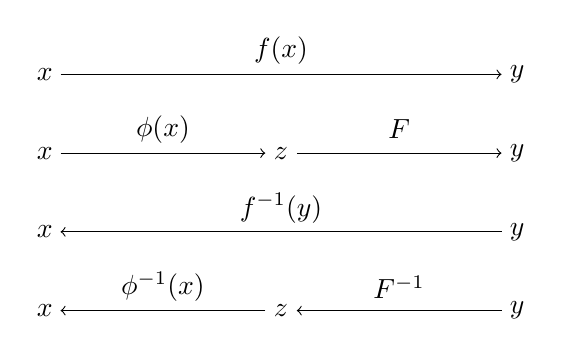
\begin{tikzpicture}
      \node[] at (0, 0) {\(x\)};
      \node[] at (0,-1) {\(x\)};
      \node[] at (0,-2) {\(x\)};
      \node[] at (0,-3) {\(x\)};

      \node[] at (6, 0) {\(y\)};
      \node[] at (6,-1) {\(y\)};
      \node[] at (6,-2) {\(y\)};
      \node[] at (6,-3) {\(y\)};

      \node[] at (3,-1) {\(z\)};
      \node[] at (3,-3) {\(z\)};
      
      \node[] at (3,   0.3) {\(f(x)\)};
      \node[] at (1.5,-0.7) {\(\phi(x)\)};
      \node[] at (4.5,-0.7) {\(F\)};
      \node[] at (3,  -1.7) {\(f^{-1}(y)\)};
      \node[] at (1.5,-2.7) {\(\phi^{-1}(x)\)};
      \node[] at (4.5,-2.7) {\(F^{-1}\)};
      
      \draw[->] (0.2, 0) -- (5.8, 0);
      \draw[->] (0.2,-1) -- (2.8,-1);
      \draw[->] (3.2,-1) -- (5.8,-1);
      \draw[->] (5.8,-2) -- (0.2,-2);
      \draw[->] (2.8,-3) -- (0.2,-3);
      \draw[->] (5.8,-3) -- (3.2,-3);
    \end{tikzpicture}
    \caption{Grafische Darstellungsform}\label{fig:beispiel3_umkehrfunktion}
  \end{figure}
